% Figure 2 (fig:claimpass, paper/sections/03-design.tex): the claim pass.
% Source: docs/02-architecture.md §2 P2, §4 step 8 and §6.6 (claim pass: every requested predicate
% for every candidate of the claim-pass pool), §6.9 step 3 (verified score); 03-design.tex §3.2-3.5.
% The predicates are names from the library; the cell values are illustrative, not a real case.
% Black plus one accent colour.
% Build: pdflatex fig2-claim-pass.tex (writes fig2-claim-pass.pdf, which \diagram includes).
\documentclass[tikz,border=2pt]{standalone}
\usepackage[T1]{fontenc}
\usetikzlibrary{positioning,arrows.meta,calc,decorations.pathreplacing}
\definecolor{accent}{RGB}{0,90,160}
\begin{document}
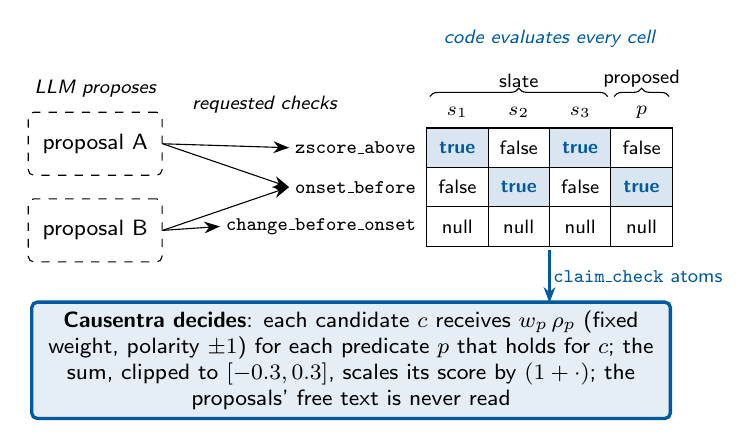
\begin{tikzpicture}[
  font=\sffamily\footnotesize,
  >={Stealth[length=2mm]},
  prop/.style={draw, dashed, rounded corners=2pt, minimum width=1.7cm, minimum height=0.8cm,
    align=center, inner sep=2pt},
  pred/.style={anchor=east, font=\ttfamily\scriptsize, inner sep=2pt},
  cell/.style={draw, minimum width=0.78cm, minimum height=0.5cm, inner sep=0pt, font=\sffamily\scriptsize},
  yes/.style={cell, fill=accent!15, text=accent, font=\sffamily\scriptsize\bfseries},
  head/.style={font=\sffamily\scriptsize, inner sep=1pt},
  tag/.style={font=\sffamily\scriptsize\itshape, inner sep=1pt},
]
% grid geometry: rows at y = 0, -0.5, -1; columns at x = 0, 0.78, 1.56, 2.34
\def\cw{0.78}
% ---------------------------------------------------------------- rows: distinct requested predicates
\node[pred] (r1) at (-0.45,0)    {zscore\_above};
\node[pred] (r2) at (-0.45,-0.5) {onset\_before};
\node[pred] (r3) at (-0.45,-1.0) {change\_before\_onset};
% ---------------------------------------------------------------- columns: claim-pass pool
\foreach \c/\lab [count=\i from 0] in {s1/$s_1$, s2/$s_2$, s3/$s_3$, p/$p$} {
  \node[head] at (\i*\cw, 0.45) {\lab};
}
\draw[decorate, decoration={brace, amplitude=3pt}] (-0.35,0.65) -- (1.91,0.65)
  node[midway, above=2pt, head] {slate};
\draw[decorate, decoration={brace, amplitude=3pt}] (1.99,0.65) -- (2.69,0.65)
  node[midway, above=2pt, head] {proposed};
% ---------------------------------------------------------------- cells: one claim_check atom each (illustrative)
\node[yes]  at (0*\cw,0)    {true};  \node[cell] at (1*\cw,0)    {false}; \node[yes]  at (2*\cw,0)    {true};  \node[cell] at (3*\cw,0)    {false};
\node[cell] at (0*\cw,-0.5) {false}; \node[yes]  at (1*\cw,-0.5) {true};  \node[cell] at (2*\cw,-0.5) {false}; \node[yes]  at (3*\cw,-0.5) {true};
\node[cell] at (0*\cw,-1.0) {null};  \node[cell] at (1*\cw,-1.0) {null};  \node[cell] at (2*\cw,-1.0) {null};  \node[cell] at (3*\cw,-1.0) {null};
% ---------------------------------------------------------------- proposals (LLM): arrows reach rows, never cells
\node[prop] (pa) at (-4.6,0.05)  {proposal A};
\node[prop] (pb) at (-4.6,-1.05) {proposal B};
\draw[->] (pa.east) -- (r1.west);
\draw[->] (pa.east) -- (r2.west);
\draw[->] (pb.east) -- (r2.west);
\draw[->] (pb.east) -- (r3.west);
% ---------------------------------------------------------------- lane tags
\node[tag, above=4pt of pa.north] {LLM proposes};
\node[tag] at (-2.45,0.55) {requested checks};
\node[tag, accent] at (1.17,1.38) {code evaluates every cell};
% ---------------------------------------------------------------- verifier
\node[draw=accent, very thick, fill=accent!10, rounded corners=2pt, align=flush center, inner sep=3pt,
  text width=7.9cm] (ce) at (-1.35,-2.7)
  {\textbf{Causentra decides}: each candidate $c$ receives $w_p\,\rho_p$ (fixed weight, polarity $\pm 1$) for each predicate $p$ that holds for $c$; the sum, clipped to $[-0.3, 0.3]$, scales its score by $(1+\cdot)$; the proposals' free text is never read};
\draw[->, thick, accent] (1.17,-1.3) -- node[right, head, text=accent] {\texttt{claim\_check} atoms} (1.17,-1.97);
\end{tikzpicture}
\end{document}
